\documentclass[paper=a5,fontsize=8pt, DIV=calc]{scrartcl}
% \documentclass[border=10pt,tikz,png]{standalone}
							
\usepackage[document]{ragged2e}
\usepackage[english]{babel}
\usepackage[utf8x]{inputenc}
\usepackage[T1]{fontenc}
\usepackage[ttdefault=true]{AnonymousPro}
\renewcommand*\familydefault{\ttdefault} %% Only if the base font of the document is to be typewriter style
\usepackage[protrusion=true,expansion=true]{microtype}
\usepackage{amsmath,amsfonts,amsthm}     % Math packages
\usepackage{graphicx}                    % Enable pdflatex
\usepackage[svgnames]{xcolor}            % Colors by their 'svgnames'
\usepackage[top=1mm, bottom=1mm, left=1mm, right=1mm]{geometry}
% 	\textheight=500px                    % Saving trees ;-)
\usepackage{tabularx,ragged2e}
\usepackage{url}
\usepackage{multicol}
\usepackage{graphicx}
\usepackage{tikz}
\usetikzlibrary{decorations.pathmorphing,shapes}
\tikzset{Warning/.style={
        rectangle,align=center,append after command={
            \pgfextra{
            \draw[ragged line,decorate,#1]
                (\tikzlastnode.north west) -- (\tikzlastnode.north east);
             \draw[ragged line,decorate,#1]
                (\tikzlastnode.south west) -- (\tikzlastnode.south east);
            }
        }
    },
    ragged line/.style={
        decoration={zigzag,amplitude=0.2mm,segment length=0.8mm}%
  }
}
\tikzset{Note/.style={
        rectangle,align=center,append after command={
            \pgfextra{
            \draw (\tikzlastnode.north west) -- (\tikzlastnode.north east);
            \draw (\tikzlastnode.south west) -- (\tikzlastnode.south east);
            }
        }
    },
}


\frenchspacing              % Better looking spacings after periods


\usepackage{hyperref}

%%% Custom sectioning (sectsty package)
%%% ------------------------------------------------------------
\usepackage{sectsty}

\sectionfont{%			            % Change font of \section command
	\usefont{OT1}{phv}{b}{n}%		% bch-b-n: CharterBT-Bold font
	\sectionrule{0pt}{0pt}{-5pt}{3pt}}

%%% Macros
%%% ------------------------------------------------------------
% \newlength{\spacebox}
% \settowidth{\spacebox}{8888888888}			% Box to align text
\newcommand{\sepspace}{\vspace*{1ex}}		% Vertical space macro


\newcommand{\TitlePage}[2]{ % Title page
        \sepspace
        \vfill
        \begin{center}
            \Huge \usefont{OT1}{phv}{b}{n} #1\\ \sepspace
            \Large \textsc{#2}\\ \vfill \normalfont
            \large by etcher\\ \vspace{1EM} \par \normalsize \vfill
            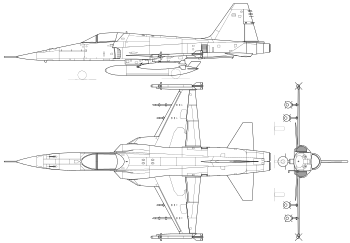
\includegraphics[width=0.5\linewidth]{title.png} \sepspace \vfill \vfill
            \Large \underline{DISCLAIMER:} Not to be used for real world operation \vfill \vfill
            \warning{This document is work in progress and is not complete as of today} \vfill \vfill
        \end{center}
        \vfill
        \raggedleft Published \today\\
        License: \href{http://creativecommons.org/licenses/by-nc-nd/4.0/}{Creative Commons Attribution-NonCommercial-NoDerivatives}\\
        \break \newpage \normalfont}
		
\renewcommand{\hline}{\noindent}

\newcommand{\oldx}[2]{%
    \item
    % \begin{minipage}{\linewidth}
    \begin{justify}
    #1 \dotfill \textsc{#2}%
    \setcounter{enumcount}{\value{enumi}}%
    \end{justify}
    % \end{minipage}
}%

\setlength\tabcolsep{1ex}
\newcommand{\x}[2]{%
    \item
    \begin{tabularx}{\linewidth}{ @{} X r @{} }
      \noindent\parbox[b]{\hsize}{#1 \dotfill} & \textsc{#2}
    \end{tabularx}
}%

\newenvironment{cl}[1]% Checklist
    {\section*{\hfill\textsc{#1}}%
    \raggedright
    \begin{enumerate}\itemsep1pt}%
    {\end{enumerate}}%

\newenvironment{clinc}% Checklist
    {\begin{enumerate}\itemsep1pt}%
    {\end{enumerate}%
}%
    
    
\newcommand{\inlinenote}[2]{%
    \begin{center}
        \begin{tikzpicture}[]%
             \node[#1]{\textsc{#1}};%
        \end{tikzpicture}
            \\ \justifying #2
            % \\ \par\noindent #2
    \end{center}
}%
    
\newcommand{\warning}[1]{\inlinenote{Warning}{#1}}%
\newcommand{\note}[1]{\inlinenote{Note}{#1}}%

\setlength{\columnseprule}{0.4pt}


%%% Begin Document
%%% ------------------------------------------------------------
\begin{document}

\TitlePage{F-5E-3}{Pocket Checklists}

\sepspace

\begin{multicols}{2}

\raggedright

\begin{cl}{Preflight}
    \x{Rudder trim}{centered}
    \x{Radar mode}{off}
    \x{Flap lever}{thumb switch}
    \x{Throttle}{cutoff}
    \x{Speed brakes}{neutral}
    \x{Flaps thumb switch}{up}
    \x{Nose strut}{retract}
    \x{Fuel shutoff left and right}{open}
    \x{Landing lights}{off}
    \x{Landing gear alternate release handle}{stowed}
    \x{Gear lever}{down}
    \x{Drag chute handle}{stowed}
    \x{Optical sight}{off}
    \warning{Power surge at generator start might damage the optical sight}
    \x{Auxiliary intake}{closed}
    \x{UHF radio}{as required}
    \x{TACAN}{as required}
    \x{Intercom}{as required}
    \x{NAV mode}{as required}
    \x{Brakes}{Check}
    \x{Pitot heat}{off}
    \x{Engine anti-ice}{off}
    \x{External fuel transfer}{off}
    \x{Fuel boost pumps LEFT and RIGHT}{on}
    \x{Fuel crossfeed}{off}
    \x{Battery}{on}
    \x{Generator left and right}{on}
    \x{Compass}{as required}
    \x{Interior lights}{as required}
    \x{NAV lights}{on}
    \x{Formation lights}{on}
    \x{Warning test}{test}
\end{cl}


\begin{cl}{Prior to engine start}
    \x{External power}{as required}
    \x{Seat height}{as required}
    \x{Danger area around aircraft}{clear}
    \x{Beacon light}{on}
\end{cl}

\note{With temperature below 10\textdegree C, an extra ignition cycle might be required before engine start}

\begin{cl}{Left engine start}
    \x{External air}{connect}
    \x{External air}{apply}
    \x{Above 10\% RPM}{start left}
    \warning{%
    If engine does not start after 5 seconds (10 seconds below minus 15\textdegree C), pull throttle back to OFF and motor engine for at least 1 minute before attempting another start.
    
    If EGT exceeds 850\textdegree C, pull throttle back to OFF and let engine cool for at least 1 minute.
    }%
    \item Check engine parameters:
    \begin{clinc}
        \x{RPM}{49 to 52\%}
        \x{EGT}{\textgreater 140\textdegree C}
        \x{Fuel flow}{$\pm$ 400pph}
        \x{Oil pressure}{5-20 PSI}
    \end{clinc}
    \x{Left generator}{on at 43\% RPM}
    \x{Utility hydraulic}{2800-3200 PSI}
\end{cl}


\begin{cl}{Right engine start}
    \x{External air}{connect}
    \x{External air}{apply}
    \x{Above 10\% RPM}{start right}
    \warning{If engine does not start after 5 seconds (10 seconds below minus 15\textdegree C), pull throttle
    back to OFF and motor engine for at least 1 minute before attempting another start \par \vspace{1em} If EGT exceeds 850\textdegree C, pull throttle back to OFF and let engine cool for at least 1 minute}
    \item Check engine parameters: \\
    \begin{clinc}
        \x{RPM}{49 to 52\%}
        \x{EGT}{\textgreater 140\textdegree C}
        \x{Fuel flow}{$\pm$ 400pph}
        \x{Oil pressure}{5-20 PSI}
    \end{clinc}
    \x{Left generator}{on at 43\% RPM}
    \x{Flight controls hydraulic}{2800-3200 PSI}
\end{cl}


\begin{cl}{Prior to taxiing}
    \x{Generator crossover}{check}
    \x{Radar mode}{standby}
    \warning{Radar operation time on the ground should not exceed 10 minutes due to the possibility of its overheating. If the radar operates on the ground for a long time, set radar mode selector to OFF. Set to STBY just before the takeoff.}
    \x{Speed brakes}{retracted}
    \x{Flaps thumb switch}{auto}
    \x{Damper switch YAW}{on}
    \x{Damper switch PITCH}{on}
    \x{Pitch damper cutoff}{actuate}
    \x{Damper switch disengaged}{check}
    \x{Damper switch PITCH}{on}
    \x{Flight controls}{check}
    \x{Takeoff trim}{set}
    \begin{minipage}{\linewidth}
        \begin{tabularx}{\textwidth}{>{\centering\raggedleft}X X}
            \textbf{Payload} & \textbf{Pitch trim} \\
            No stores & 6 \\
            Gun, missiles  & 7 \\
            Bombs, rockets & 9
        \end{tabularx}
    \end{minipage}
    \x{Aileron trim}{check}
    \x{Rudder trim}{check}
    \x{Altimeter}{check}
    \x{Wheel chocks}{removed}
    \x{Landing light}{on}
\end{cl}


\begin{cl}{Taxi}
    \x{Wheel brakes}{release}
    \x{NWS}{engage}
    \x{Trottle}{70\% until moving}
    \x{Wheel brakes}{check}
    \x{Trottle}{70\% until moving}
    \x{Throttle}{Reduce to 57\%}
\end{cl}

\begin{cl}{Prior to takeoff}
    \x{Optical sight mode}{as required}
    \x{Radar mode}{as required}
    \x{Pitot heat}{on}
    \x{Engine anti ice}{as required}
    \x{IFF}{as required}
    \x{Canopy}{close}
    \x{Warning panel}{no light on}
    \note{Engine anti-ice light might be on is selected}
    \x{Nose strut}{extend}
\end{cl}

\newpage

\begin{cl}{Takeoff}
    \x{Instruments}{check}
    \x{Wheel brakes}{applied}
    \x{Throttles}{MIL}
    \item Instruments
    \begin{enumerate}
        \x{Acceleration time}{7 seconds}
        \x{RPM}{101 $\pm$ 2\%}
        \x{Stabilization time}{10 seconds}
        \x{EGT}{665-675\textdegree C}
        \x{Nozzle position}{0-16\%}
    \end{enumerate}
    \x{Wheel brakes}{release}
    \x{Throttle}{max}
    \x{Steering}{differential brakes}
    \x{Liftoff minus 10 KIAS}{Pull}
    \begin{minipage}{\linewidth}
        \begin{tabularx}{\textwidth}{>{\centering\raggedleft}X X >{\centering\raggedleft}X X}
            \textbf{Weight} & \textbf{Liftoff} & \textbf{Weight} & \textbf{Liftoff}\\
            \textless 15000 & 143-145 &  21000             & 168-175 \\
             16000          & 153-155 &  22000             & 178-180 \\
             18000          & 164-168 & \textgreater 23000 & 185-190 \\
             19000          & 166-168 &  
        \end{tabularx}
    \end{minipage}
    \x{Climb rate}{positive}
    \x{Airspeed}{increasing}
    \x{Landing gear}{up}
    \x{Trim}{as required}
    \x{Flaps}{as required}
    \x{Aux doors closed}{check}
\end{cl}

\begin{cl}{Climb}
    \x{Speed}{\textgreater 280kts}
    \x{Fuel transfer}{as required}
\end{cl}

\begin{cl}{Approach}
    \x{Fuel transfer}{off}
    \x{Fuel}{check}
    \x{Altimeter}{check}
    \x{Landing lights}{on}
    \x{Hydraulic}{2800 to 3200 psi}
    \x{Aux intake door (\textless300KIAS \& \textless3000ft)}{open}
    \x{3 miles before RWY}{300KIAS \& 1500ft}
    \x{Flaps thumb Sw}{auto}
    \x{Flaps lever}{thumb sw}
    \x{Speed}{260KIAS}
    \x{Gear}{down, 3 green}
    \x{Downwind}{165KIAS \& 1500ft}
    \x{AOA}{on speed}
    \x{Final}{-1000ft/min}
    \begin{minipage}{\linewidth}
        \begin{tabularx}{\textwidth}{>{\centering\raggedleft}X X}
            \textbf{Fuel left} & \textbf{Speed}\\
            4000 & 160 \\
            3000 & 155 \\
            2000 & 150 \\
            1000 & 145
        \end{tabularx}
        \note{With gun ammunition onboard, add 5 knots to approachelanding speed}
    \end{minipage}
\end{cl}

\begin{cl}{After landing}
    \x{Cockpit pressurization}{ram dump}
    \x{Flaps switch}{up}
    \x{Radar mode}{off}
    \x{Optical sight}{off}
    \x{Pitot heat and engine anti-ice}{off}
    \x{Rotating beacon}{on}
\end{cl}

\begin{cl}{Engine shutdown}
    \x{Wheel chocks}{install}
    \x{Canopy}{open}
    \x{Cockpit pressurization}{normal}
\end{cl}


\end{multicols}
\end{document}
